\begin{frame}{Camera Pose: Six Degrees of Freedom}
  \begin{columns}[T,onlytextwidth]
    \column{0.47\textwidth}
      \begin{itemize}\footnotesize\itemsep0.3em
        \item \textbf{Camera pose:} the rigid transform $(R,\mathbf{t})\in SE(3)$, $\mathbf{X}_c=R\,\mathbf{X}_w+\mathbf{t}$: six DoF, three for rotation and three for translation.
        \item \textbf{Relative pose} links two cameras (from $E$, with $\mathbf{t}$ only up to scale). \textbf{Absolute pose} places one camera in a fixed map frame; this section estimates it.
        \item Human pose estimation (body keypoints) is a different task.
        \item \textbf{Quaternion:} $q=(q_w,q_x,q_y,q_z)=q_w+q_x\,i+q_y\,j+q_z\,k$ with $i^2=j^2=k^2=ijk=-1$. The rotation by angle $\theta$ about the unit axis $\mathbf{n}$ is the unit quaternion $q=\big(\cos\tfrac{\theta}{2},\ \mathbf{n}\sin\tfrac{\theta}{2}\big)$.
        \item \textbf{Why networks regress quaternions:} any nonzero 4-vector becomes a valid rotation after division by its norm, which is simpler than projecting a $3\times3$ output onto $SO(3)$.
      \end{itemize}
    \column{0.51\textwidth}
      \centering
      {\scriptsize\setlength{\tabcolsep}{3pt}
      \begin{tabular}{>{\raggedright\arraybackslash}p{1.55cm} p{0.75cm} >{\raggedright\arraybackslash}p{4.1cm}}
        \toprule
        \textbf{Rotation as} & \textbf{Count} & \textbf{Constraint and catch} \\
        \midrule
        Matrix $R$ & 9 & $R^\top R=I$, $\det R=+1$: six constraints, so a raw network output is not a rotation \\
        \addlinespace[0.2em]
        Euler angles & 3 & three turns about coordinate axes, e.g.\ yaw, pitch, roll (vertical, sideways, forward axis); gimbal lock: at pitch $\pm90^\circ$ the yaw and roll axes align and one DoF is lost \\
        \addlinespace[0.2em]
        Axis--angle $\theta\mathbf{n}$ & 3 & minimal, but $\pi\mathbf{n}$ and $-\pi\mathbf{n}$ are the same rotation \\
        \addlinespace[0.2em]
        Unit quaternion $q$ & 4 & one constraint, $\lVert q\rVert=1$; no singularities; $q$ and $-q$ are the same rotation \\
        \bottomrule
      \end{tabular}\par}
      \vspace{0.6em}
      \begin{itemize}\footnotesize\itemsep0.3em
        \item \textbf{The catch:} $\theta\to\theta+2\pi$ flips the sign of $q$, so every rotation has two labels. Either make labels unique, e.g.\ store each with $q_w>0$, plus a sign rule for half-turns ($q_w=0$), or use a loss that treats $q$ and $-q$ as equal, e.g.\ $\min(\lVert q^{*}-q\rVert,\lVert q^{*}+q\rVert)$ for the label $q^{*}$.
      \end{itemize}
  \end{columns}
\end{frame}

\begin{frame}{Perspective-n-Point (PnP)}
  \begin{columns}[T,onlytextwidth]
    \column{0.54\textwidth}
      \begin{itemize}\footnotesize\itemsep0.3em
        \item \textbf{Problem:} given $K$ and $n$ matches $\mathbf{x}_i\leftrightarrow\mathbf{X}_i$ from pixels to known 3D map points, find $R,\mathbf{t}$ with $\lambda_i\tilde{\mathbf{x}}_i=K\,[R\mid\mathbf{t}]\,\tilde{\mathbf{X}}_i$. Six unknowns and two equations per match: three matches are the minimum.
        \item \textbf{P3P} (three matches): the unknowns are the distances $d_i=\lVert\mathbf{X}_i-\mathbf{C}\rVert$. The map gives $D_{ij}=\lVert\mathbf{X}_i-\mathbf{X}_j\rVert$; $K$ gives the angle $\theta_{ij}$ between the rays $\hat{\mathbf{x}}_i,\hat{\mathbf{x}}_j$, where $\hat{\mathbf{x}}=K^{-1}\tilde{\mathbf{x}}$. The law of cosines,
        \[ D_{ij}^2=d_i^2+d_j^2-2\,d_i d_j\cos\theta_{ij},\qquad i<j\in\{1,2,3\}, \]
        has at most four solutions with positive $d_i$; a fourth point or the RANSAC inlier count picks one.
        \item \textbf{EPnP ($n\geq4$):} $\mathbf{X}_i=\sum_{j=1}^{4}\alpha_{ij}\mathbf{c}_j$ with four virtual control points $\mathbf{c}_j$. Their 12 camera-frame coordinates come from the eigenvectors of a $12\times12$ matrix, in $O(n)$ time.
        \item \textbf{In practice:} a minimal solver inside RANSAC, then reprojection-error refinement on the inliers. At inlier ratio $w=0.5$ and confidence $p=0.99$, RANSAC needs 35 samples of size $s=3$, or 72 of size $s=4$.
      \end{itemize}
    \column{0.44\textwidth}
      \centering
      \begin{tikzpicture}[font=\sffamily\scriptsize, >=latex,
          x={(0.47cm,0.27cm)}, y={(0cm,0.8cm)}, z={(0.8cm,0cm)},
          dot/.style={circle, fill, inner sep=1.1pt}]
        % Camera frame: centre at the origin, image plane at depth f = 2.2.
        % Image points are x_i = (f/Z_i) X_i, so each lies exactly on its ray and on the plane.
        \coordinate (C) at (0,0,0);
        \coordinate (X1) at (-0.3,1.9,4.6);
        \coordinate (X2) at (1.5,0.3,5.4);
        \coordinate (X3) at (-0.9,-1.5,4.2);
        \fill[blue!8] (-1.25,-1.25,2.2) -- (1.25,-1.25,2.2) -- (1.25,1.25,2.2) -- (-1.25,1.25,2.2) -- cycle;
        \draw[blue!60!black] (-1.25,-1.25,2.2) -- (1.25,-1.25,2.2) -- (1.25,1.25,2.2) -- (-1.25,1.25,2.2) -- cycle;
        \fill[orange!14] (X1) -- (X2) -- (X3) -- cycle;
        \draw[orange!70!black, dashed] (X1) -- (X2) -- (X3) -- cycle;
        \draw[gray!70!black] (C) -- (X1);
        \draw[gray!70!black] (C) -- (X2);
        \draw[gray!70!black] (C) -- (X3);
        \coordinate (x1) at ($(C)!0.478261!(X1)$);
        \coordinate (x2) at ($(C)!0.407407!(X2)$);
        \coordinate (x3) at ($(C)!0.523810!(X3)$);
        \node[dot, blue!70!black] at (x1) {};
        \node[dot, blue!70!black] at (x2) {};
        \node[dot, blue!70!black] at (x3) {};
        \node[dot] at (C) {};
        \node[dot, orange!80!black] at (X1) {};
        \node[dot, orange!80!black] at (X2) {};
        \node[dot, orange!80!black] at (X3) {};
        \draw[thick] ($(C)!0.85cm!(X1)$) to[bend left=35] ($(C)!0.85cm!(X3)$);
        \node at ($(C)+(0.62cm,-0.1cm)$) {$\theta_{13}$};
        \node[left] at (C) {$\mathbf{C}$};
        \node[above left] at (X1) {$\mathbf{X}_1$};
        \node[right] at (X2) {$\mathbf{X}_2$};
        \node[below right] at (X3) {$\mathbf{X}_3$};
        \node[blue!70!black, above left, inner sep=1.5pt] at (x1) {$\mathbf{x}_1$};
        \node[blue!70!black, below right, inner sep=1.5pt] at (x2) {$\mathbf{x}_2$};
        \node[blue!70!black, below left, inner sep=2pt] at (x3) {$\mathbf{x}_3$};
        \node[above, sloped] at ($(C)!0.72!(X1)$) {$d_1$};
        \node[below, sloped] at ($(C)!0.72!(X3)$) {$d_3$};
        \node[orange!70!black, left] at ($(X1)!0.5!(X3)$) {$D_{13}$};
        \node[blue!60!black, anchor=north west] at (-1.25,-1.25,2.2) {image plane};
      \end{tikzpicture}\\[0.3em]
      {\scriptsize Each ray from the camera centre $\mathbf{C}$ through an image point $\mathbf{x}_i$ meets its map point $\mathbf{X}_i$. The triangle $\mathbf{C}\mathbf{X}_1\mathbf{X}_3$ gives the P3P equation for $(i,j)=(1,3)$.\par}
      \vspace{0.5em}
      {\scriptsize Solution count: Gao et al., ``Complete Solution Classification for the Perspective-Three-Point Problem,'' IEEE TPAMI 25(8), 2003, \href{https://doi.org/10.1109/TPAMI.2003.1217599}{doi:10.1109/TPAMI.2003.1217599}. Lepetit, Moreno-Noguer and Fua, ``EPnP: An Accurate O(n) Solution to the PnP Problem,'' IJCV 81(2), 2009, \href{https://doi.org/10.1007/s11263-008-0152-6}{doi:10.1007/s11263-008-0152-6}.\par}
  \end{columns}
\end{frame}

\begin{frame}{Visual Localization: Retrieve, Match, Solve}
  \begin{columns}[T,onlytextwidth]
    \column{0.43\textwidth}
      \begin{itemize}\footnotesize\itemsep0.3em
        \item \textbf{Map, built offline} by structure from motion (SfM, next slides): images with known poses, their local features, 3D points, and one global descriptor per image.
        \item \textbf{Retrieve:} the query's global descriptor finds the $k$ nearest map images (image retrieval), grouped into places by the 3D points they share.
        \item \textbf{Match:} query keypoints are matched only to the 3D points of each place.
        \item \textbf{Solve:} PnP inside RANSAC gives the 6-DoF pose; the search stops at the first place with a valid pose.
        \item \textbf{Uses:} relocalizing an AR device in a pre-mapped room, or a robot in a prebuilt map.
      \end{itemize}
    \column{0.55\textwidth}
      \centering
      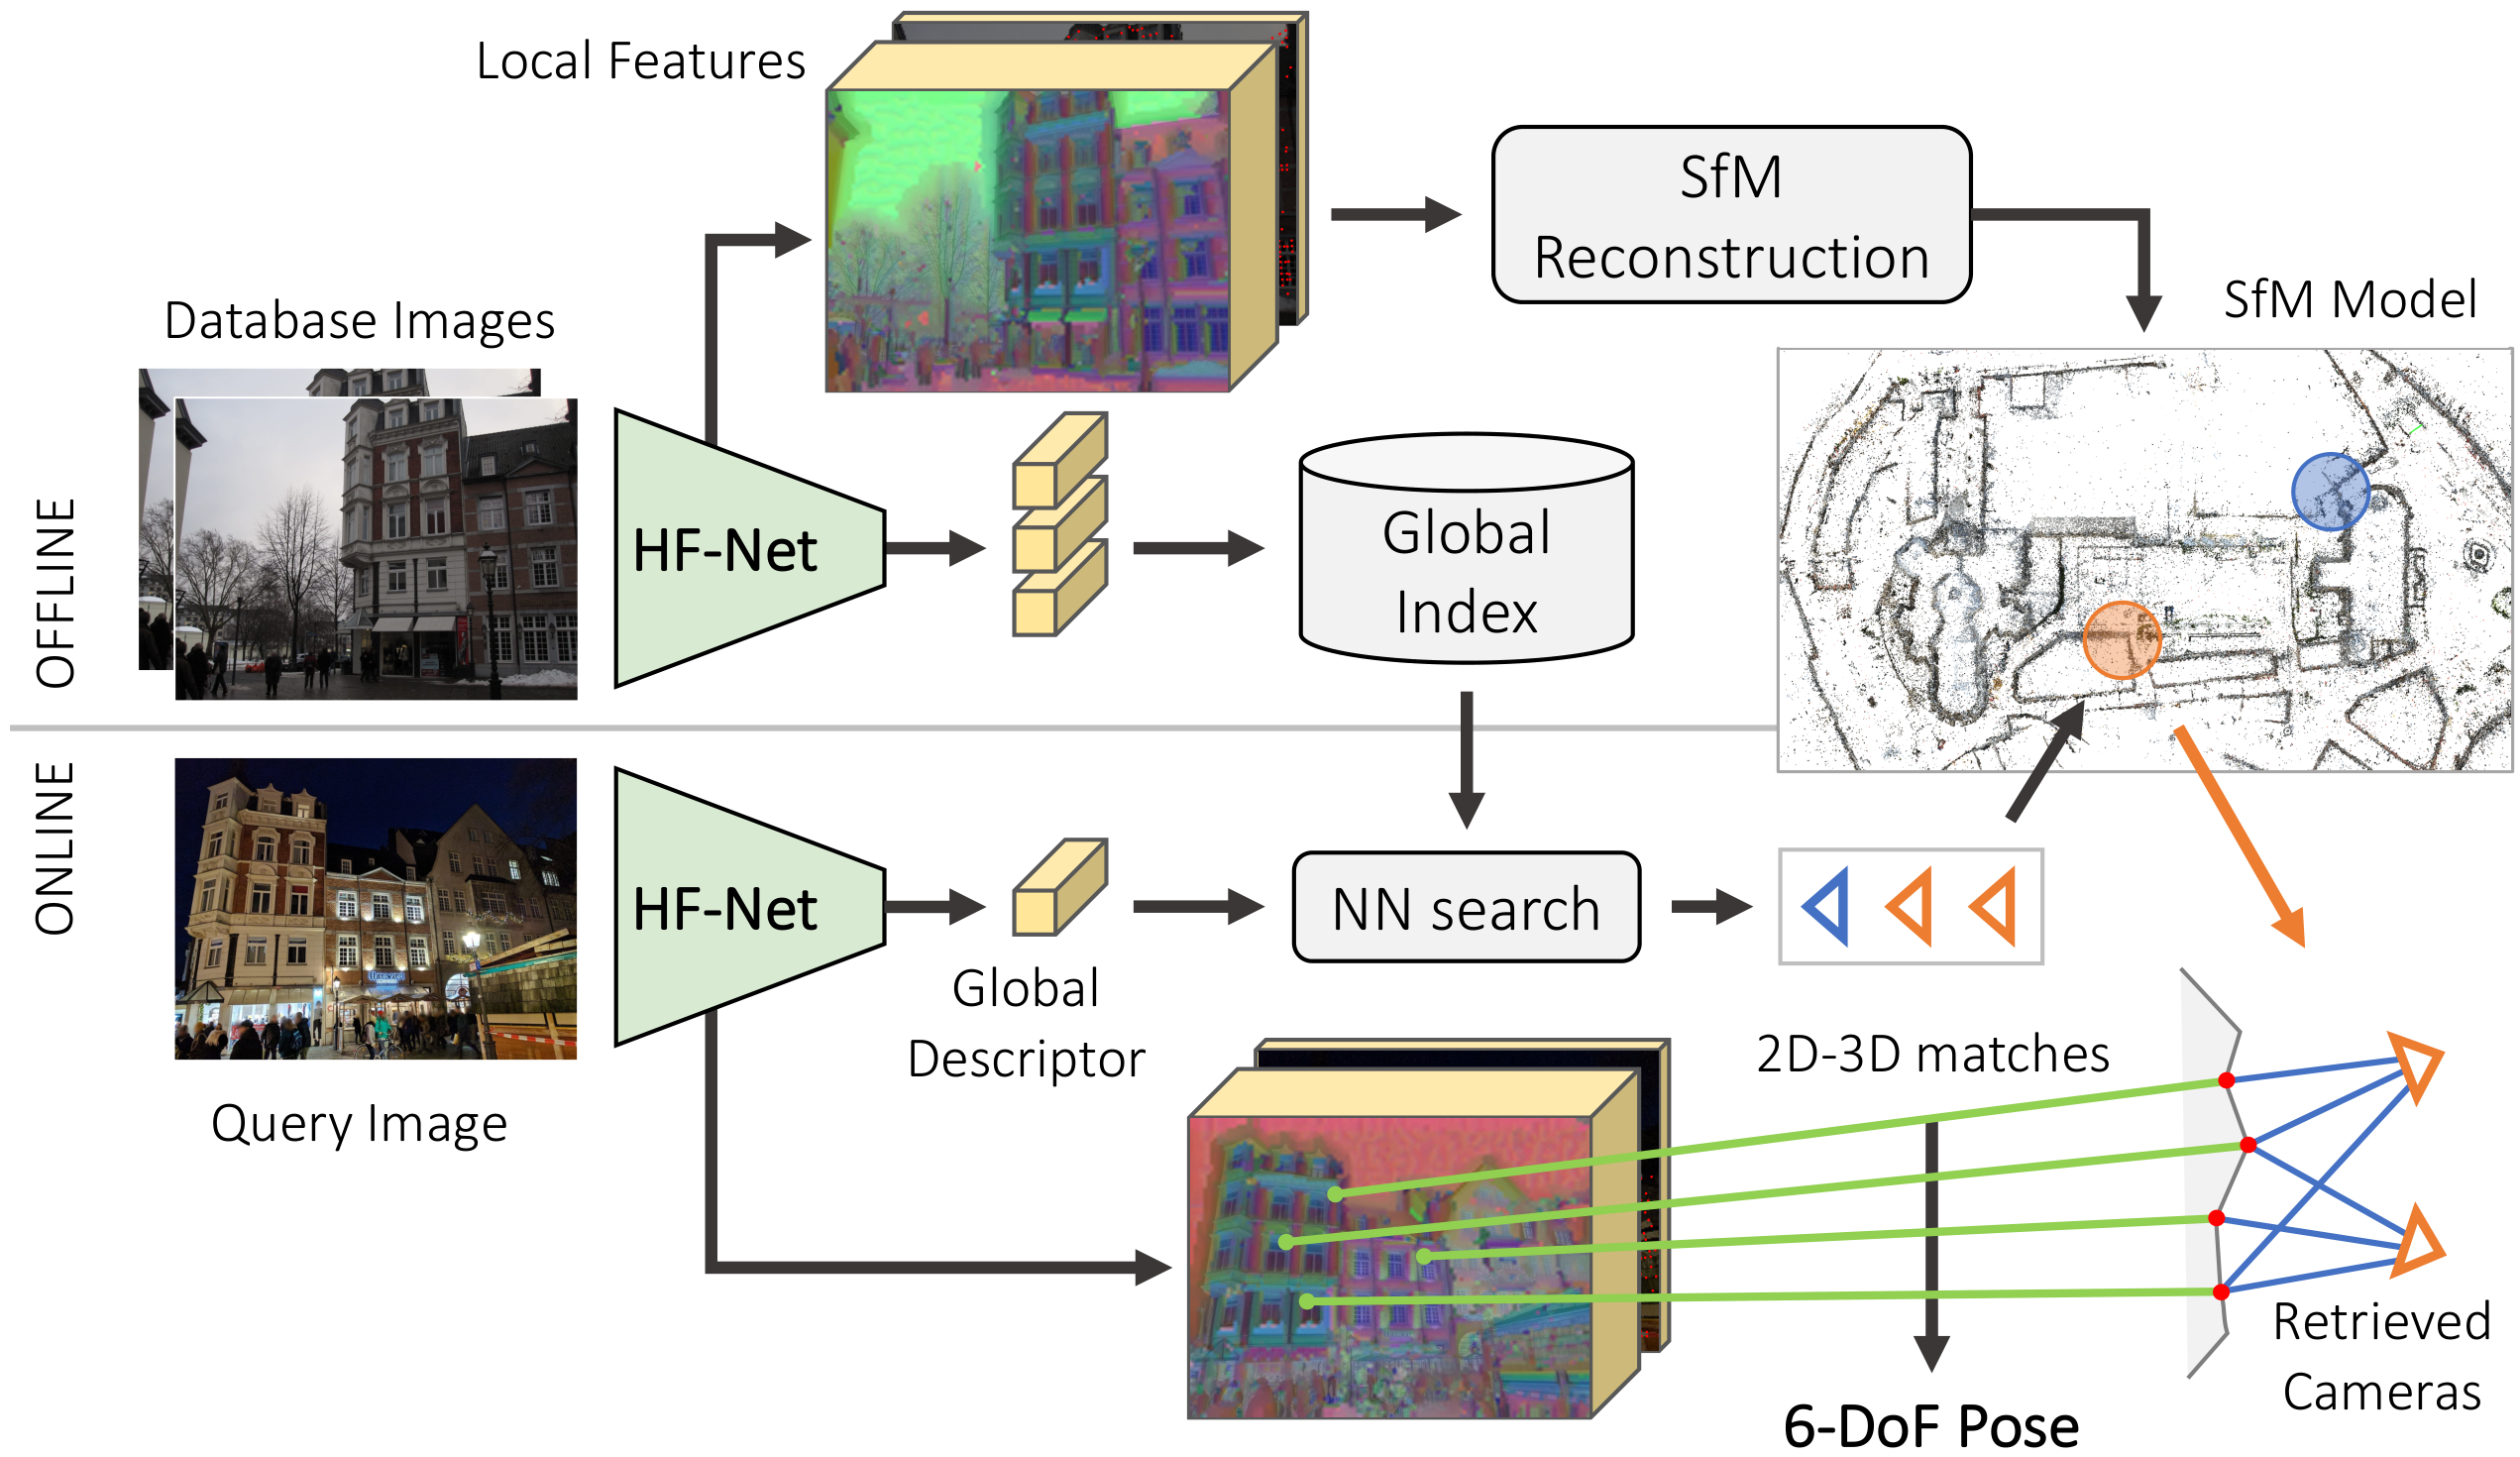
\includegraphics[width=\linewidth,height=0.5\textheight,keepaspectratio]{images/3d-vision/hloc_fig2_hierarchical_localization.png}\\[0.2em]
      {\scriptsize Sarlin et al., ``From Coarse to Fine: Robust Hierarchical Localization at Large Scale,'' CVPR 2019, \href{https://arxiv.org/abs/1812.03506v2}{arXiv:1812.03506v2}, Figure~2; numbers from Table~3 and Sections~5.3--5.4.\par}
      \vspace{0.4em}
      \begin{itemize}\scriptsize\itemsep0.2em
        \item \textbf{Retrieval alone is coarse:} for the 98 night-time queries of Aachen Day-Night (map: 4,328 daytime images of a European old town), the top retrieved image's pose is within 0.5\,m and $2^\circ$ for 0.0\%; retrieve, match and solve reaches 40.8\% (NetVLAD global descriptor, SuperPoint features).
        \item HF-Net computes the global descriptor and local features in one network; the pipeline runs at 20 frames per second.
      \end{itemize}
  \end{columns}
\end{frame}

\begin{frame}{Regressing Pose Directly, and Its Limits}
  \begin{columns}[T,onlytextwidth]
    \column{0.55\textwidth}
      \begin{itemize}\footnotesize\itemsep0.25em
        \item \textbf{PoseNet:} a CNN regresses the camera position $\mathbf{C}$ and a quaternion $q$ from one image in 5\,ms, trained on poses from SfM:
        \[ \mathcal{L}=\lVert\mathbf{C}^{*}-\mathbf{C}\rVert_2+\beta\,\Big\lVert q^{*}-\frac{q}{\lVert q\rVert}\Big\rVert_2 \]
        $\mathbf{C},q$: outputs; $\mathbf{C}^{*},q^{*}$: ground truth; $\beta$ balances metres against quaternion units (grid search: 120--750 indoors, 250--2000 outdoors).
        \item \textbf{The limit:} the last layer is linear, so the output $\mathbf{b}+\sum_j\alpha_j(I)\,\mathbf{p}_j$ is a weighted sum of learned base poses $\mathbf{p}_j$; trained on cameras along a line, it predicts poses on that line. Pose regression is ``more closely related to pose approximation via image retrieval than to accurate pose estimation via 3D structure.''
        \item \textbf{Scene coordinate regression:} predict the 3D scene point seen at each pixel (or patch), then run PnP inside RANSAC. DSAC* trains end to end through a differentiable RANSAC; ACE trains only an MLP head on a fixed backbone: 291\,s of mapping against 15\,h for DSAC* on one V100 GPU, a 4\,MB map, and accuracy on par.
      \end{itemize}
    \column{0.43\textwidth}
      \centering
      {\scriptsize King's College (outdoor, $140\times40$\,m, Cambridge Landmarks), median error\par}
      \vspace{0.2em}
      {\scriptsize\setlength{\tabcolsep}{3pt}
      \begin{tabular}{l l r}
        \toprule
        \textbf{Approach} & \textbf{Method} & \textbf{m / deg} \\
        \midrule
        Pose regression & PoseNet & 1.92 / 5.40 \\
        Image retrieval & DenseVLAD & 2.80 / 5.72 \\
                        & + interpolation & 1.48 / 4.45 \\
        2D--3D matching & Active Search & 0.42 / 0.55 \\
        Scene coordinates & DSAC++ & 0.18 / 0.3 \\
        \bottomrule
      \end{tabular}\par}
      \vspace{0.2em}
      {\scriptsize + interpolation: poses of the top 20 retrieved images, weighted to best reproduce the query's descriptor.\par}
      \vspace{0.3em}
      {\scriptsize Sattler et al., ``Understanding the Limitations of CNN-based Absolute Camera Pose Regression,'' CVPR 2019, \href{https://arxiv.org/abs/1903.07504v1}{arXiv:1903.07504v1}, Table~2, Eq.~3, Section~5.\par}
      \vspace{0.3em}
      {\scriptsize Kendall et al., ``PoseNet: A Convolutional Network for Real-Time 6-DOF Camera Relocalization,'' ICCV 2015, \href{https://arxiv.org/abs/1505.07427v4}{arXiv:1505.07427v4}, Eq.~2, Figure~6. Brachmann and Rother, ``Visual Camera Re-Localization from RGB and RGB-D Images Using DSAC,'' TPAMI 2021, \href{https://arxiv.org/abs/2002.12324v4}{arXiv:2002.12324v4}. Brachmann et al., ``Accelerated Coordinate Encoding: Learning to Relocalize in Minutes using RGB and Poses,'' CVPR 2023, \href{https://arxiv.org/abs/2305.14059v1}{arXiv:2305.14059v1}, Table~3.\par}
  \end{columns}
\end{frame}

\begin{frame}{Structure from Motion: The Incremental Pipeline}
  \centering
  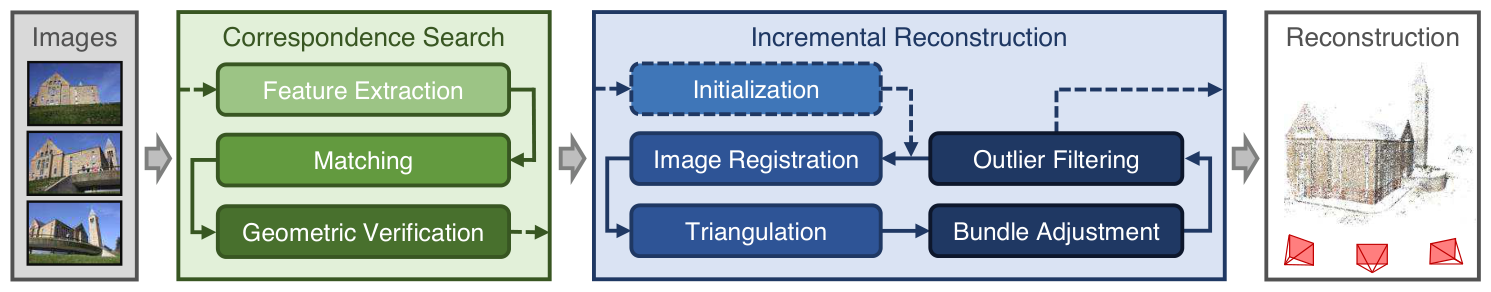
\includegraphics[width=\textwidth,height=0.27\textheight,keepaspectratio]{images/3d-vision/colmap_fig2_incremental_sfm_pipeline.png}\\[0.2em]
  {\scriptsize Sch\"onberger and Frahm, ``Structure-from-Motion Revisited,'' CVPR 2016, \href{https://doi.org/10.1109/CVPR.2016.445}{doi:10.1109/CVPR.2016.445}, Figure~2 (COLMAP).\par}
  \vspace{0.4em}
  \begin{columns}[T,onlytextwidth]
    \column{0.49\textwidth}
      \begin{itemize}\footnotesize\itemsep0.3em
        \item \textbf{Input:} unordered photos of a scene. \textbf{Output:} intrinsics $K_i$, poses $(R_i,\mathbf{t}_i)$, and a sparse point cloud of 3D points $\mathbf{X}_j$, each point with the pixels $\mathbf{x}_{ij}$ that observe it.
        \item \textbf{Correspondence search:} features (SIFT or learned), matching, and geometric verification with RANSAC on $E$, $F$ or $H$. Verified pairs form the scene graph: images are nodes, pairs are edges.
        \item \textbf{Initialization:} relative pose and triangulation on a carefully chosen pair in a densely connected part of the graph, because ``the reconstruction may never recover from a bad initialization.''
      \end{itemize}
    \column{0.49\textwidth}
      \begin{itemize}\footnotesize\itemsep0.3em
        \item \textbf{Registration:} the next image is located by PnP inside RANSAC from its 2D--3D matches to points already in the model.
        \item \textbf{Triangulation} adds the new points it sees; \textbf{bundle adjustment} (next slide) refines cameras and points jointly; \textbf{outlier filtering} drops observations with large reprojection error.
        \item ``Without further refinement, SfM usually drifts quickly to a non-recoverable state.'' COLMAP, the open-source system of this paper, adjusts locally after every registration and globally each time the model has grown by a set percentage.
      \end{itemize}
  \end{columns}
\end{frame}

\begin{frame}{Bundle Adjustment}
  \begin{columns}[T,onlytextwidth]
    \column{0.54\textwidth}
      \begin{itemize}\footnotesize\itemsep0.25em
        \item \textbf{Objective:} refine all cameras and points jointly,
        \[ \min_{\{K_i,R_i,\mathbf{t}_i\},\,\{\mathbf{X}_j\}}\ \sum_{(i,j)\in\mathcal{V}}\rho\Big(\big\lVert\mathbf{x}_{ij}-\pi(K_i,R_i,\mathbf{t}_i,\mathbf{X}_j)\big\rVert^2\Big) \]
        $\mathcal{V}$: observed (image, point) pairs. $\rho$: a robust loss of the squared residual $e$: Huber, $e$ for $e\leq\delta^2$ and $2\delta\sqrt{e}-\delta^2$ above, or Cauchy, $\delta^2\log(1+e/\delta^2)$ (COLMAP uses it in local adjustment). Both grow slower than $e$, so a wrong match pulls less.
        \item \textbf{Levenberg--Marquardt (LM):} residuals $\mathbf{r}(\boldsymbol{\theta})$ over all parameters $\boldsymbol{\theta}$, Jacobian $J=\partial\mathbf{r}/\partial\boldsymbol{\theta}$. Each step solves $(J^\top J+\mu I)\,\Delta\boldsymbol{\theta}=-J^\top\mathbf{r}$. If the cost drops, accept and shrink $\mu$ (toward Gauss--Newton, the exact step for linearized $\mathbf{r}$); if not, grow $\mu$ ($\Delta\boldsymbol{\theta}\approx-J^\top\mathbf{r}/\mu$, a short gradient-descent step).
        \item \textbf{Gauge freedom:} a similarity transform of the whole scene ($3+3+1=7$ DoF) changes no residual, so $J^\top J$ is singular: fix the first camera and the scale.
      \end{itemize}
      \vspace{0.1em}
      {\scriptsize Triggs, McLauchlan, Hartley and Fitzgibbon, ``Bundle Adjustment: A Modern Synthesis,'' Vision Algorithms: Theory and Practice, LNCS 1883, 2000, \href{https://doi.org/10.1007/3-540-44480-7_21}{doi:10.1007/3-540-44480-7\_21}, Sections~6.1 and~9.\par}
    \column{0.44\textwidth}
      \centering
      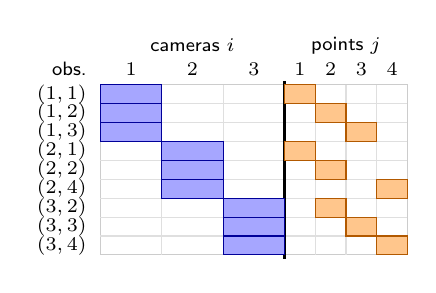
\begin{tikzpicture}[font=\sffamily\scriptsize, >=latex,
          cam/.style={fill=blue!35, draw=blue!60!black},
          pt/.style={fill=orange!45, draw=orange!70!black}]
        % Columns: a camera block is 0.78 cm wide (6 pose parameters), a point block 0.39 cm (3 coordinates).
        % Rows: one block row of height 0.24 cm per observation (i,j).
        \draw[gray!40] (0,0) rectangle (3.9,-2.16);
        \foreach \r in {1,...,8} \draw[gray!25] (0,-0.24*\r) -- (3.9,-0.24*\r);
        \foreach \c in {0.78,1.56,2.73,3.12,3.51} \draw[gray!25] (\c,0) -- (\c,-2.16);
        \draw[thick] (2.34,0.05) -- (2.34,-2.21);
        \foreach \r/\i/\j in {0/1/1, 1/1/2, 2/1/3, 3/2/1, 4/2/2, 5/2/4, 6/3/2, 7/3/3, 8/3/4} {
          \draw[cam] ({0.78*(\i-1)},{-0.24*\r}) rectangle ({0.78*\i},{-0.24*(\r+1)});
          \draw[pt] ({2.34+0.39*(\j-1)},{-0.24*\r}) rectangle ({2.34+0.39*\j},{-0.24*(\r+1)});
          \node[anchor=east] at (-0.05,{-0.24*\r-0.12}) {$(\i,\j)$};
        }
        \foreach \i in {1,2,3} \node at ({0.78*\i-0.39},0.2) {$\i$};
        \foreach \j in {1,2,3,4} \node at ({2.34+0.39*\j-0.195},0.2) {$\j$};
        \node at (1.17,0.5) {cameras $i$};
        \node at (3.12,0.5) {points $j$};
        \node[anchor=east] at (-0.05,0.2) {obs.};
      \end{tikzpicture}\\[0.2em]
      {\scriptsize Sparsity of $J$: each residual involves one camera and one point.\par}
      \vspace{0.3em}
      {\scriptsize\raggedright
      \textbf{Schur complement:} split $J^\top J+\mu I$ into $U$ (cameras), $V$ (points) and $W$ (coupling), and $-J^\top\mathbf{r}$ into $\mathbf{g}_c$, $\mathbf{g}_p$. $V$ is block diagonal ($3\times3$ per point), so $V^{-1}$ is cheap. Eliminating the points leaves the reduced camera system
      \[ (U-WV^{-1}W^\top)\,\Delta\boldsymbol{\theta}_c=\mathbf{g}_c-WV^{-1}\mathbf{g}_p, \]
      small because cameras are far fewer than points; $U-WV^{-1}W^\top$ is the Schur complement of $V$. Then $\Delta\boldsymbol{\theta}_p=V^{-1}(\mathbf{g}_p-W^\top\Delta\boldsymbol{\theta}_c)$.\par}
  \end{columns}
\end{frame}

\begin{frame}{Global SfM: GLOMAP}
  \centering
  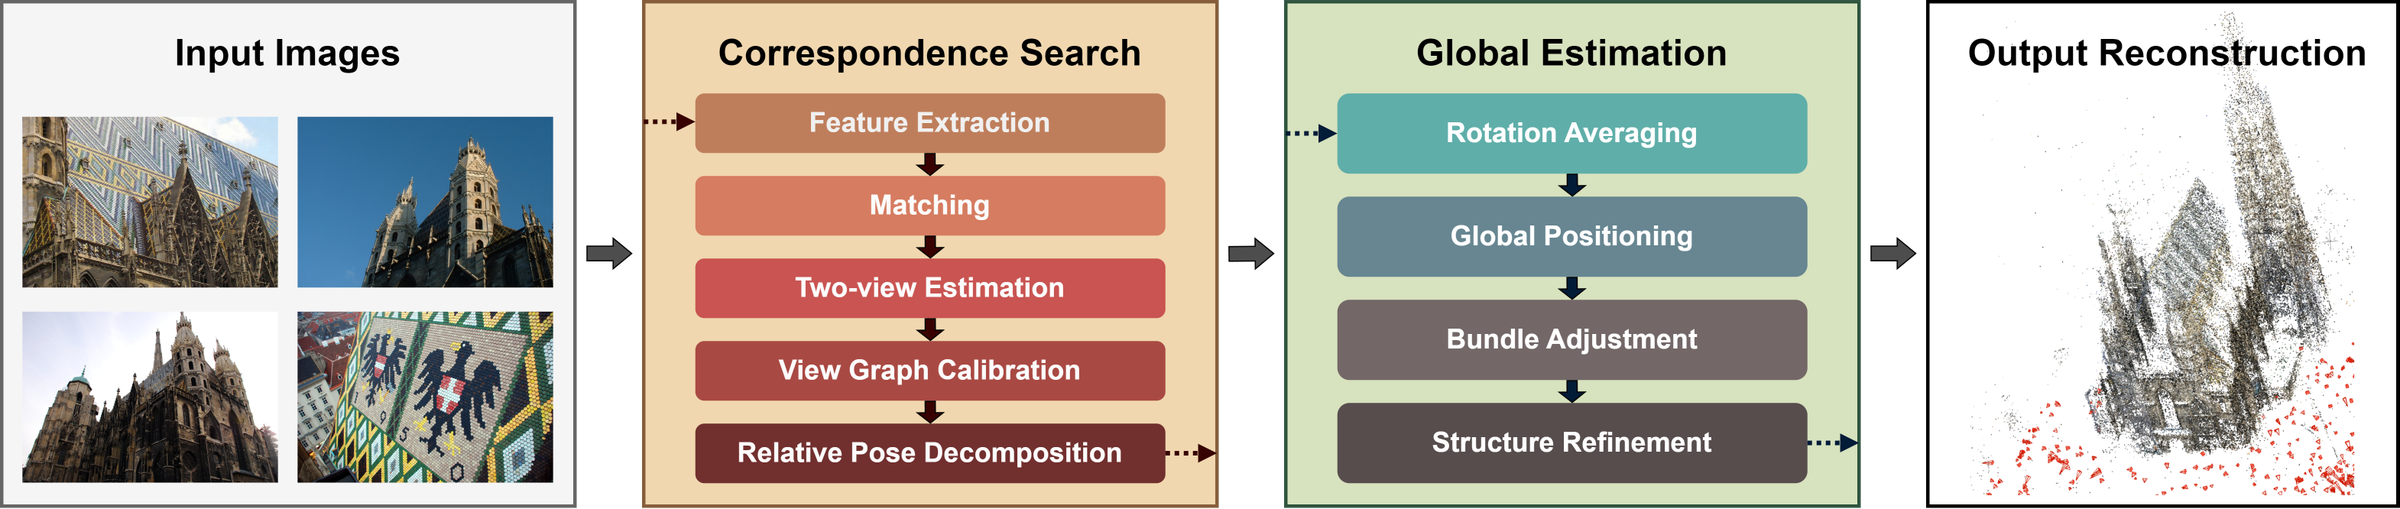
\includegraphics[width=\textwidth,height=0.35\textheight,keepaspectratio]{images/3d-vision/glomap_fig2_global_sfm_pipeline.png}\\[0.2em]
  {\scriptsize Pan et al., ``Global Structure-from-Motion Revisited,'' ECCV 2024, \href{https://arxiv.org/abs/2407.20219v2}{arXiv:2407.20219v2}, Figure~2, Sections~1, 2.2, Eqs.~3--4.\par}
  \vspace{0.1em}
  \begin{columns}[T,onlytextwidth]
    \column{0.42\textwidth}
      \begin{itemize}\footnotesize\itemsep0.3em
        \item \textbf{Global SfM} solves all cameras at once. \textbf{Rotation averaging} fits every $R_i$ to the pairwise rotations of the scene graph, $R_{ij}\approx R_jR_i^\top$, with outliers down-weighted. Positions, triangulation and bundle adjustment follow.
        \item Positions usually come from \textbf{translation averaging} of the pairwise directions $\mathbf{t}_{ij}$, which lack scale and degenerate under nearly collinear motion.
      \end{itemize}
    \column{0.56\textwidth}
      \begin{itemize}\footnotesize\itemsep0.3em
        \item \textbf{GLOMAP} replaces translation averaging and triangulation with one global positioning of camera centres $\mathbf{C}_i$ and points $\mathbf{X}_k$:
        \[ \min_{\mathbf{X},\,\mathbf{C},\,s}\ \sum_{i,k}\rho\big(\lVert\mathbf{v}_{ik}-s_{ik}(\mathbf{X}_k-\mathbf{C}_i)\rVert_2\big),\ \ s_{ik}\geq0 \]
        $\mathbf{v}_{ik}$: unit world-frame ray direction from camera $i$ to point $k$; $s_{ik}$: a free scale. With the best $s_{ik}$ the error is the sine of the angle between the two rays, capped at 1, so outliers stay bounded; random initialization converges.
      \end{itemize}
  \end{columns}
\end{frame}

\begin{frame}{Incremental Versus Global SfM}
  \centering
  {\scriptsize
  \begin{tabular}{>{\raggedright\arraybackslash}p{1.7cm} >{\raggedright\arraybackslash}p{5.2cm} >{\raggedright\arraybackslash}p{5.2cm}}
    \toprule
    & \textbf{Incremental (COLMAP)} & \textbf{Global (GLOMAP)} \\
    \midrule
    Speed & bundle adjustment repeated as the model grows & adjustment rounds only at the end \\
    \addlinespace[0.15em]
    Robustness & each new image must pass PnP with RANSAC; a bad seed pair can ruin the run & fails when rotation averaging fails, e.g.\ in symmetric scenes \\
    \addlinespace[0.15em]
    Drift & accumulates along the registration order & all pairwise constraints are used at once \\
    \addlinespace[0.15em]
    Typical use & the standard general-purpose tool & large collections and long sequences \\
    \bottomrule
  \end{tabular}\par}
  \vspace{0.8em}
  \begin{columns}[T,onlytextwidth]
    \column{0.56\textwidth}
      \centering
      {\scriptsize\setlength{\tabcolsep}{3pt}
      \begin{tabular}{l l r r r}
        \toprule
        \textbf{Data} & \textbf{Measure} & \textbf{GLOMAP} & \textbf{COLMAP} & \textbf{Theia} \\
        \midrule
        ETH3D SLAM & recall, 0.1\,m (\%) & 66.4 & 57.9 & 62.8 \\
                   & time (s) & 133.5 & 1115.4 & 91.8 \\
        LaMAR & recall, 1\,m (\%) & 49.1 & 32.0 & 11.0 \\
              & time (s) & 12{,}405 & 354{,}660 & 1{,}542 \\
        \bottomrule
      \end{tabular}\par}
    \column{0.42\textwidth}
      \begin{itemize}\scriptsize\itemsep0.2em
        \item \textbf{Recall:} \% of cameras whose position, after aligning the reconstruction to the ground truth, is within the threshold; averaged over scenes.
        \item \textbf{Times} exclude feature extraction and matching, which all methods share.
        \item \textbf{ETH3D SLAM:} video sequences with sparse features, moving objects and strong lighting changes. \textbf{LaMAR:} tens of thousands of AR-device images per scene. \textbf{Theia:} another global system.
      \end{itemize}
  \end{columns}
  \vspace{0.5em}
  {\scriptsize Pan et al., \href{https://arxiv.org/abs/2407.20219v2}{arXiv:2407.20219v2}, Sections~1, 2.5, 3.3, 4 and~4.4, Tables~1 and~4. Incremental column: Sch\"onberger and Frahm, CVPR 2016, Sections~2.2 and~4.4.\par}
\end{frame}
